\documentclass{article}
\usepackage{amsmath}
\usepackage{graphicx}
\usepackage{bm} %for bold lower greek symbols

\title{Feed Forward Neural Network}
\author{Masahiro Ogawa}

\begin{document}
\maketitle

\section{Notation}
\begin{itemize}
\item $\bm{x}$ : vector
\item $\bm{A}$ : matrix
\item ${}^t\bm{A}$ : transpose of $\bm{A}$
\item $f.(\bm{A}) = 
 \begin{pmatrix}
  f(a_{1,1}) & f(a_{1,2}) & \cdots & f(a_{1,n}) \\
  f(a_{2,1}) & f(a_{2,2}) & \cdots & f(a_{2,n}) \\
  \vdots  & \vdots  & \ddots & \vdots  \\
  f(a_{m,1}) & f(a_{m,2}) & \cdots & f(a_{m,n})
 \end{pmatrix}$ 
\item $(\bm{A}.*\bm{B})_{i,j} = a_{i,j}b_{i,j}$
\item $\bm{1}_{m\times n} = 
  \begin{pmatrix}
    1 & \cdots & 1 \\
    \vdots & \ddots & \vdots \\
    1 & \cdots & 1 
  \end{pmatrix}$ : $m \times n$ dim
\item $\bm{\tilde{y}} = 
  \begin{pmatrix}
    1 \\
    \bm{y}
  \end{pmatrix}$ : homogeneous vector
\item $n$ : data number
\item $N$ : total number of data
\item $l$ : layer number
\item $L$ : output layer number. thus, the total number of layer is $L+1$
\item $k$ : learning iteration number
\item $K$ : final number of the learning iteration 
\item $J$ : cost
\item $f(x)$ : activation function
\item $\bm{X}_0 = (\bm{x}_{0,1},\dots , \bm{x}_{0,N}) = 
  \begin{pmatrix}
    x_{0,1,1} & \cdots & x_{0,1,N} \\
    \vdots & \ddots & \vdots\\
    x_{0,d_0,1} & \cdots & x_{0,d_0,N}
  \end{pmatrix}$
  : $d_0 \times N$ dim : input vectors
\item $\bm{B} = (\bm{b}_1,\dots , \bm{b}_N) =
  \begin{pmatrix}
    b_{1,1} & \cdots & b_{1,N}\\
    \vdots & \ddots & \vdots\\
    b_{d_L,1} & \cdots & b_{d_L,N}
  \end{pmatrix}
  $ : $d_L \times N$ dim : instruction signals
\item $\bm{\tilde{W}}_l(k) =
  (\bm{\tilde{w}}_{l,1}(k),\dots , \bm{\tilde{w}}_{l,d_{l+1}}(k)) = 
  \begin{pmatrix}
    \tilde{w}_{l,0,1}(k) & \cdots & \tilde{w}_{l,0,d_{l+1}}(k)\\
    \vdots & \ddots & \vdots\\
    \tilde{w}_{l,d_l,1}(k) & \cdots & \tilde{w}_{l,d_l,d_{l+1}}(k)
  \end{pmatrix}
  $ :
  weights : $(d_l+1) \times d_{l+1}$ dim 
\end{itemize}


\section{Input}
parameters
\begin{itemize}
\item $L$ : output layer number.
\item $\{ d_l \}_{l=0}^L$ : neuron numbers in each layer $l$
\item $\{\bm{\tilde{W}}_l(0)\}_{l=0}^L \mid \bm{\tilde{W}}_l(0) =
  (\bm{\tilde{w}}_{l,1}(0),\dots , \bm{\tilde{w}}_{l,d_{l+1}}(0))$ :
  $(d_l+1) \times d_{l+1}$ dim : initial weights
\item $\rho$ : learning rate parameter
\item $T_e$ : error threshold
\item $T_K$ : threshold of the maximum number of iteration
\end{itemize}

data 
\begin{itemize}
\item $\bm{X}_0 = (\bm{x}_{0,1},\dots , \bm{x}_{0,N})$ : $d_0 \times N$ dim : input vectors
\item $\bm{B} = (\bm{b}_1,\dots , \bm{b}_N)$ : $d_L \times N$ dim : instruction signals
\end{itemize}


\section{Output}
\begin{itemize}
\item $\{\bm{\tilde{W}}_l(K)\}_{l=0}^L \mid \bm{\tilde{W}}_l(K) = (\bm{\tilde{w}}_{l,1}(K),\dots ,
  \bm{\tilde{w}}_{l,d_{l+1}}(K))$ : $(d_l+1) \times d_{l+1}$ dim :
  final (after $K$th iteration) learned weights
\item $\bm{Y}_L = (\bm{y}_{L,1},\dots , \bm{y}_{L,N})$ :
  $dL \times N$ dim : output vectors
\item $J = \sum_{n=1}^N J_n$
  : cost, final error
\end{itemize}

\section{Algorithm(Iterative version, Stochastic Gradient descent)}
\begin{figure}
  \centering
  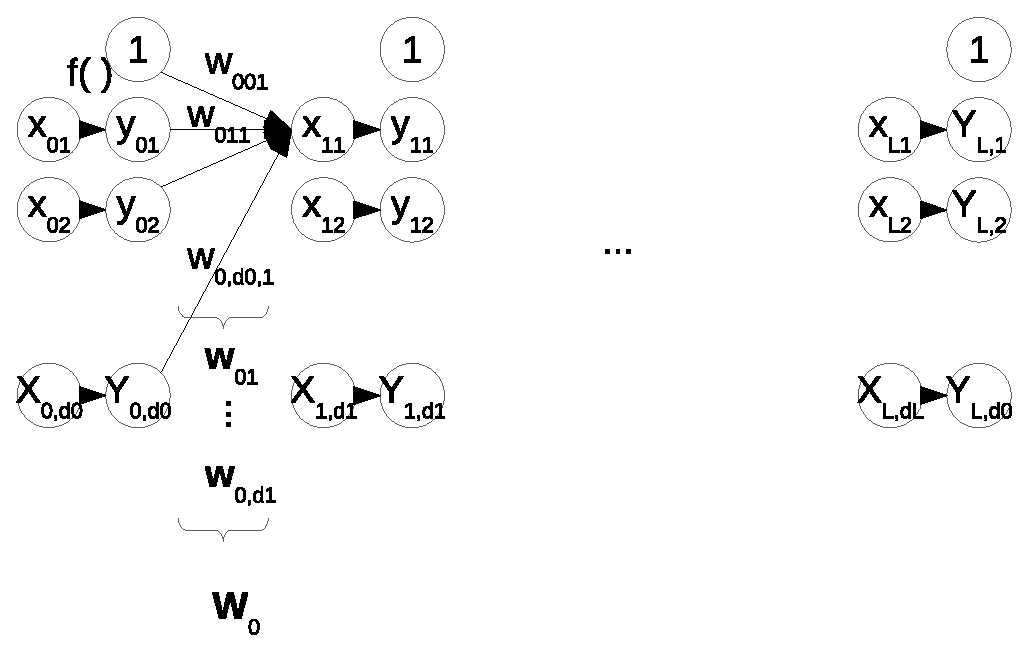
\includegraphics[width=1.0\textwidth]{neuralnet_architecture}
  \caption{Neural network architecture}
  \label{fig:nn}
\end{figure}
\subsection{Iteration}
Iterate feed forward and back propagation algorithm for each input
datum until the error become smaller than the threshold or the
iteration number exceeds the
maximum iteration number. 
That is, 
\begin{equation}
  J < T_e \mbox{, or } k < T_K.
\end{equation}

The iteration means update of the weights as,
\begin{eqnarray}
  \tilde{w}_{lij}(k+1) 
  = \tilde{w}_{lij}(k) - \rho \frac{\partial J_n}{\partial
    \tilde{w}_{lij}(k)} \\
 \iff \bm{\tilde{W}}_l(k+1) 
  = \bm{\tilde{W}}_{l}(k) - \rho \frac{\partial J_n}{\partial
    \bm{\tilde{W}}_{l}(k)} \label{eq:weight_update}
\end{eqnarray}
From this equation, once we could compute $\frac{\partial J_n}{\partial
  \bm{\tilde{W}}_{l}(k)}$, we can update the weights.
Therefore we concentrate on computing $\frac{\partial J_n}{\partial
  \bm{\tilde{W}}_{l}(k)}$ below.

\subsection{Feed Forward}
The below are true for all data and all iteration.
So we omit the data number $n$ and iteration number $k$ as 
e.g.\ $\bm{x}_{l,n} = \bm{x}_l, \bm{\tilde{W}}_l(k) = \bm{\tilde{W}}_l$.
\begin{eqnarray}
  \bm{x}_l = {}^t\bm{\tilde{W}}_{l-1} \bm{\tilde{y}}_{l-1} \\
  \bm{y}_l = f.(\bm{x}_l) \\
\end{eqnarray}

\subsubsection{activation function for hidden layers}
\begin{eqnarray}
  f(x) = 
  \begin{cases}
    (1+e^{-x})^{-1} \mbox{ : logistic function}\\
    \tanh(x) 
  \end{cases} \label{eq:activation hidden}
\end{eqnarray}

\subsubsection{activation function for an output layer}
To fit output value as desired, we have to choose appropriate activation
function for an output layer.
\begin{eqnarray}
  f(x) = 
  \begin{cases}
    x &\mbox{: identity function for regression}\\
    (1+e^{-x})^{-1} &\mbox{: logistic function for [0,1] output binary
    classification}\\
  \frac{\exp(x)}{\sum_j \exp(x_{Lj})} &\mbox{: soft max function for multiclass
  classification}\\
    \tanh(x) &\mbox{: for [-1,1] output}
  \end{cases} \label{eq:activation out}
\end{eqnarray}
Note that we divide binary and multiclass case, because if we use soft
max function for binary class classification, $f(x)$ always become 1.

\subsection{Back Propagation}
In this section, we compute $\frac{\partial J_n}{\partial
  \bm{\tilde{W}}_{l-1}(k)}$ instead of $\frac{\partial J_n}{\partial
  \bm{\tilde{W}}_{l}(k)}$ for just index convenience.
And we omit $n$ as $J_n = J$ in this section.

\begin{eqnarray}
  \frac{\partial J}{\partial \tilde{w}_{l-1,ij}}
  &=& \frac{\partial J}{\partial x_{lj}} \frac{\partial x_{lj}}{\partial
    \tilde{w}_{l-1,ij}} \\
  &=& \epsilon_{lj} \frac{\partial (\sum_m{\tilde{w}_{l-1,mj}
      \tilde{y}_{l-1,m}})}{\partial \tilde{w}_{l-1,ij}}
  \hspace{5mm} \mid \epsilon_{lj} :=  \frac{\partial J}{\partial x_{lj}}\\
  &=& \epsilon_{lj} \tilde{y}_{l-1,i}\\
  \iff \frac{\partial J}{\partial \bm{\tilde{W}}_{l-1}}
  &=& \bm{\tilde{y}}_{l-1} {}^t\bm{\epsilon_{l}}\\
  \Rightarrow \bm{\tilde{W}}_{l-1}(k+1) &=& \bm{\tilde{W}}_{l-1}(k) - \rho \bm{\tilde{y}}_{l-1}{}^t\bm{\epsilon}_l\\
  \epsilon_{lj} &=&  \frac{\partial J}{\partial x_{lj}}\\
  &=& \frac{\partial J}{\partial y_{lj}} \frac{\partial
    y_{lj}}{\partial x_{lj}}\\
  &=& \frac{\partial J}{\partial y_{lj}} \frac{\partial
    f(x_{lj})}{\partial x_{lj}}\\
\end{eqnarray}

\subsubsection{back propagation for hidden layers}
\begin{eqnarray}
  \epsilon_{lj} 
  &=& \frac{\partial J}{\partial y_{lj}} \frac{\partial
    f(x_{lj})}{\partial x_{lj}}\\
  &=& \sum_h \frac{\partial J}{\partial x_{l+1,h}} \frac{\partial
      x_{l+1,h}}{\partial y_{lj}} f'({x}_{lj})\\
  &=& \sum_h \epsilon_{l+1,h} 
    \frac{(\sum_m w_{lmh}y_{lm} + w_{l0h})}{\partial y_{lj}}  f'({x}_{lj})\\
  &=& \sum_h \epsilon_{l+1,h} w_{ljh}  f'({x}_{lj})\\
  \Rightarrow 
  \bm{\epsilon}_l &=& (\bm{W}_l\bm{\epsilon}_{l+1}) .* f'.(\bm{x}_l)\\
  &=&
  \begin{cases}
    (\bm{W}_l \bm{\epsilon}_{l+1}).*(\bm{y}_l-\bm{y}_l.*\bm{y}_l)
    &\mbox{if } f(x)=(1+e^{-x})^{-1}\\
    (\bm{W}_l \bm{\epsilon}_{l+1}).*(\bm{1}_{dl}-\bm{y}_l.*\bm{y}_l)
    &\mbox{if } f(x)=\tanh(x)
  \end{cases}
\end{eqnarray}

\subsubsection{back propagation for an output layer}
To compute back propagation for an output layer, we need cost function form.
Depend on that, we have to choose appropriate cost function for each
problem as below.
\begin{eqnarray}
  J = 
  \begin{cases}
    \frac{1}{2} \lVert \bm{y}_L-\bm{b} \rVert ^2  &\mbox{regression }\\ 
    -(b \ln y_L + (1-b)\ln(1-y_L)) &\mbox{binary classification} \\
    -{}^t\bm{b} \ln \bm{y}_L &\mbox{multiclass classification} 
  \end{cases} \label{eq:J}
\end{eqnarray}

Using cost(\ref{eq:J}) and activation function(\ref{eq:activation out}),
$\epsilon_L$ can be computed as below.
Note that $f(x_h)$ is related to $x_j$, so we have to think about the term
$\frac{\partial f(x_{Lh})}{\partial x_{Lj}}$.
\begin{eqnarray}
  \epsilon_{Lj} 
  &=& \sum_h \frac{\partial J}{\partial y_{Lh}} \frac{\partial
    f(x_{Lh})}{\partial x_{Lj}}\\
  &=&
  \begin{cases}
    \sum_h (\frac{\partial (1/2 \lVert \bm{y}_L-\bm{b} \rVert ^2)}{\partial
      y_{Lh}}) \frac{\partial x_{Lh}}{\partial x_{Lj}}
    &\mbox{regression }\\
    -(\frac{b}{y_L} - \frac{1-b}{1-y_L}) \frac{\partial}{\partial
      x_{L}}(1+e^{-x_L})^{-1}   &\mbox{binary classification}\\
    -\sum_h \frac{b_h}{y_{L,h}} \frac{\partial}{\partial
      x_{Lj}}(\frac{\exp(x_{Lh})}{\sum_i \exp(x_{Li})})
    &\mbox{multiclass classification}
  \end{cases} \\
  &=&
  \begin{cases}
    \sum_h (y_{Lh}-b_h) \delta_{h,j}\\
    -(\frac{b}{y_L} - \frac{1-b}{1-y_L})(y_L(1-y_L))\\
    -\sum_h \frac{b_h}{y_{L,h}} (\delta_{h,j}y_{Lj} - y_{Lh}y_{Lj})
  \end{cases}\\
  &=&  y_{Lj}-b_j
\end{eqnarray}
We use the softmax property $\sum_h b_h = 1$ in the last equation of multi-class
classification case.

In both case the result becomes $y-b$, so there is no gradient
diminishing problem. That's why we use these combination of the cost and
final layers activation function. 

\subsubsection{final result}
Finally, we get below results.
\begin{eqnarray}
  \bm{\epsilon}_l &=&
  \begin{cases}
    \bm{y}_L - \bm{b}  &\mbox{if } l=L \\
    (\bm{W}_l\bm{\epsilon}_{l+1}) .* f'.(\bm{x}_l) &\mbox{otherwise}
  \end{cases} \\
  &=& 
  \begin{cases}
    \bm{y}_L - \bm{b}\\
    (\bm{W}_l \bm{\epsilon}_{l+1}).*(\bm{1}_{dl}-\bm{y}_l.*\bm{y}_l)  &\mbox{if } f(x)=\tanh(x)
  \end{cases} \\
  \bm{\tilde{W}}_{l-1}(k+1) &=& \bm{\tilde{W}}_{l-1}(k) - \rho\ \bm{\tilde{y}}_{l-1}{}^t\bm{\epsilon}_l
\end{eqnarray}


\section{Algorithm(Matrix version)}
\subsection{Iteration}
Iterate feed forward algorithm for all input
data and back propagation for all data until the error become smaller than the threshold or the
iteration number exceeds the
maximum iteration number. 
That is, 
\begin{equation}
  J < T_e \mbox{, or } k < T_K.
\end{equation}

\subsection{Feed Forward}
The below are true for all iteration.
So we omit the iteration number as 
e.g.\ $\bm{\tilde{W}}_l(i) = \bm{\tilde{W}}_l$.
\begin{eqnarray}
  \bm{X}_l = {}^t\bm{\tilde{W}}_{l-1} \bm{\tilde{Y}}_{l-1} \\
  \bm{Y}_l = f.(\bm{X}_l) 
\end{eqnarray}
$f(x)$ is defined by (\ref{eq:activation hidden}) and (\ref{eq:activation
out}).

\subsection{Back Propagation}
\begin{eqnarray}
J &=&   
\begin{cases}
  \frac{1}{2} \mathrm{Tr} ({}^t(\bm{Y}_L - \bm{B})(\bm{Y}_L - \bm{B}))
  &\mbox{regression} \\
  -\mathrm{Tr} \{
  \begin{pmatrix}
    {}^t\bm{B} \\
    \bm{1}_{1 \times N} - {}^t\bm{B}
  \end{pmatrix}
  \ln. ( \bm{Y}_L \hspace{3mm}  \bm{1}_{N \times 1} - \bm{Y}_L) \} &\mbox{binary classification}\\ 
  -\mathrm{Tr} ({}^t\bm{B} \ln.(\bm{Y}_L)) &\mbox{multiclass classification}
  \end{cases}\\
  \bm{E}_l = (\bm{\epsilon}_{l,1}, \cdots, \bm{\epsilon}_{l,N}) &=&
  \begin{cases}
    \bm{Y}_L - \bm{B}  &\mbox{if } l=L \\
    (\bm{W}_l\bm{E}_{l+1}) .* f'.(\bm{X}_l) &\mbox{otherwise}
  \end{cases} \\
  &=&
  \begin{cases}
    \bm{Y}_L - \bm{B} \\
    (\bm{W}_l\bm{E}_{l+1}).*(\bm{1}_{dl\times N}-\bm{Y}_l.*\bm{Y}_l) &\mbox{if } f(x)=\tanh(x)
  \end{cases} \\
  \bm{\tilde{W}}_{l-1}(k+1) &=& \bm{\tilde{W}}_{l-1}(k) - \rho
  \sum_{n=1}^N \bm{\tilde{y}}_{l-1,n} {}^t\bm{\epsilon}_{l,n}\\
  &=& \bm{\tilde{W}}_{l-1}(k) - \rho\ \bm{\tilde{Y}}_{l-1} {}^t\bm{E}_l
\end{eqnarray}

\end{document}
